\documentclass[14pt]{article}
\usepackage{graphicx}
\usepackage[left=3cm, right=1.5cm, top=1.5cm, bottom=2cm]{geometry}
\usepackage[russian]{babel}
\usepackage[T2A]{fontenc}
\usepackage[utf8]{inputenc}
\usepackage[unicode]{hyperref}
\usepackage{a4wide}

\begin{document}
\thispagestyle{empty}
\begin{center}
	\ \vspace{-4cm}\\
	
\includegraphics[width=0.5\textwidth]{../img/msu.png}\\
	{\scshape Московский государственный университет имени М.~В.~Ломоносова}\\
	Факультет вычислительной  математики и кибернетики\\
	\vfill
	{\LARGE Задание по системам управления проектами}\\
	\vspace{1cm}
	{\Huge\bfseries <<Работа в MS Project>>}\\
	{\Huge Вариант 5} 
\end{center}
\vspace{1cm}
\begin{flushright}
	\large
	\textit{Задание выполнил}\\
	Гусейнов Али Эльшанович\\
	\vspace{5mm}
	\textit{Преподаватель}\\
	Абрамов Владимир Геннадьевич
\end{flushright}
\vfill
\begin{center}
	Москва, 2024
\end{center}
\clearpage
\tableofcontents
\clearpage
\section{Команда}
\section{Ресурсы}
	\subsection{Сетевой график}
	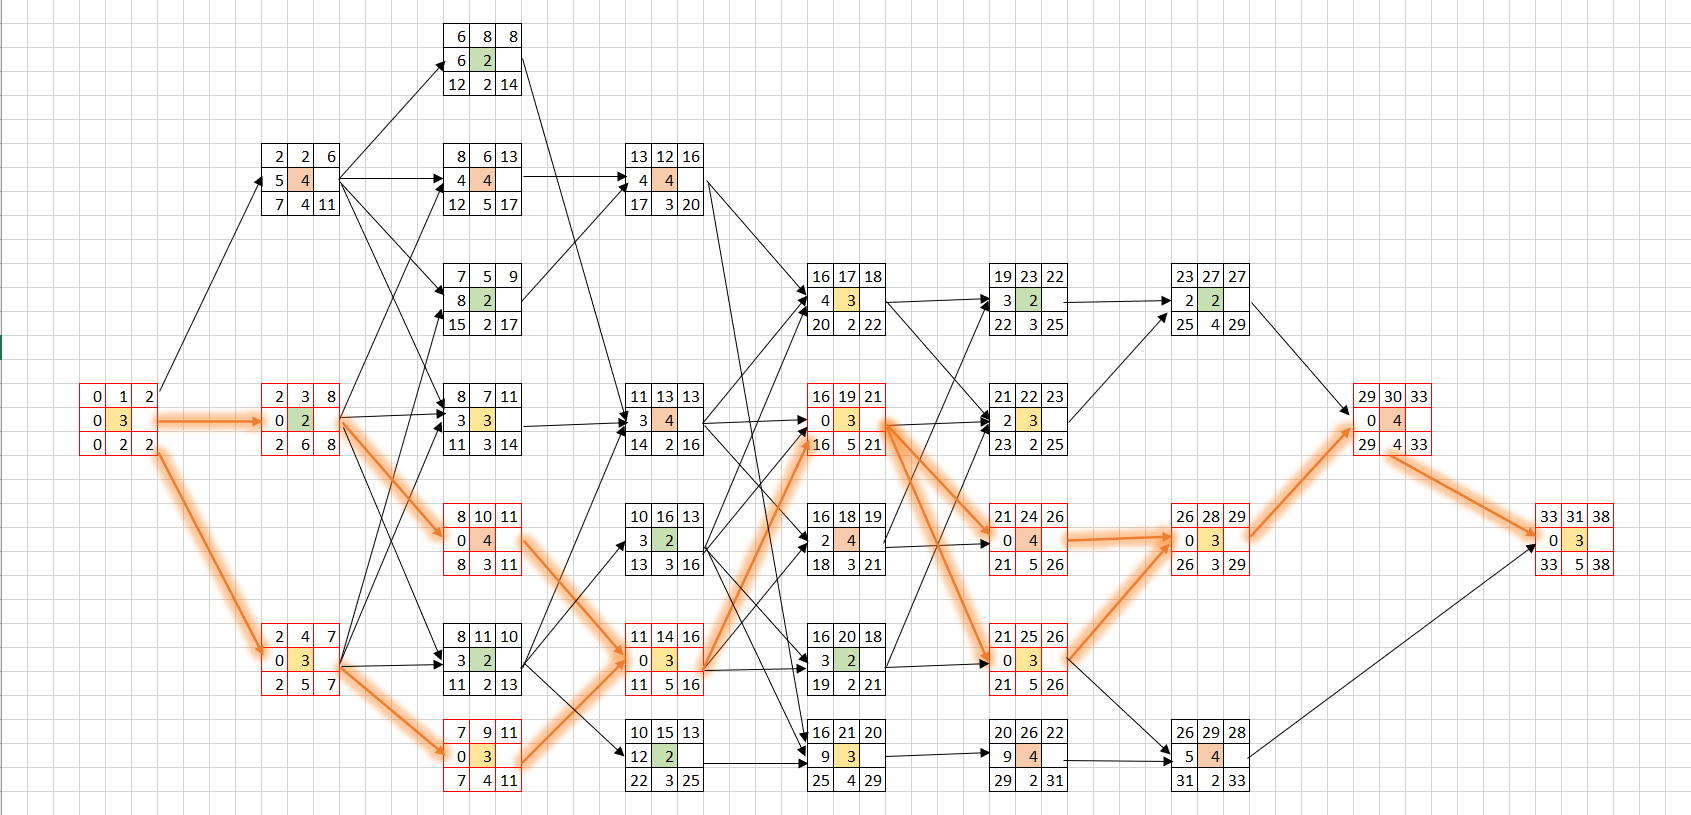
\includegraphics[width=\textwidth]{../img/init_network_graph.png}
	\subsection{Назначение ресурсов}
	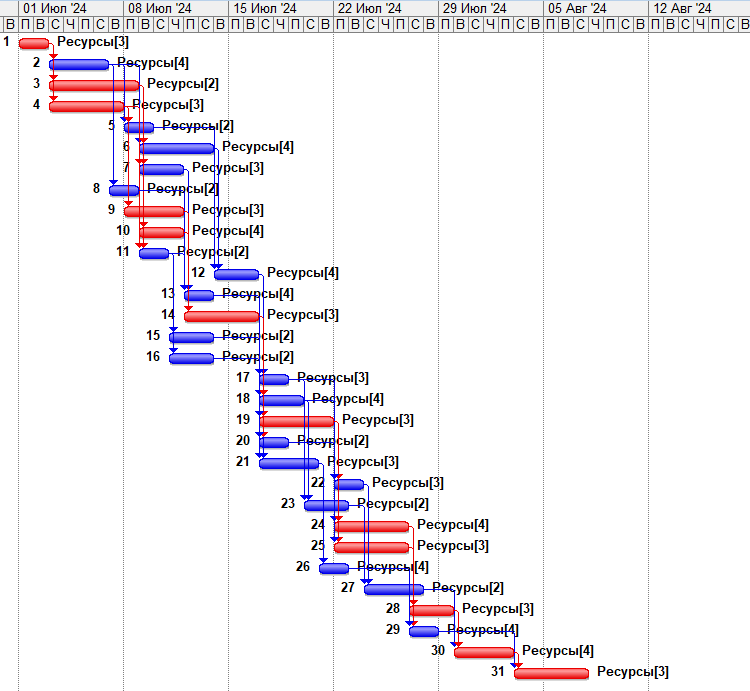
\includegraphics[width=\textwidth]{../img/init_resource_manage.png}
\section{Первый способ}
	
\end{document}
